\begin{center}
	\Huge \textbf{Собственно, матстат...}
\end{center}
\section{Функції від випадкових величин (векторів)}
Для дискретної випадкової величини $\xi$: $\eta = \phi (\xi) \Rightarrow \eta$ - ДВВ. \\
Припустимо, що $\varphi$ - неперервно диференційована. $\xi$ - асолютно неперервна зі щільністю $f_{\xi}(x)$. Розглядаємо $ \eta = \varphi(\xi) $:

\begin{boxteo}
    Нехай $\varphi$ - взаємно-однозначна (бієкція на області значень), та її обернена $\psi$ є неперервно диференційована. (Дифеоморфізм). Тоді:
    $$
    f_{\eta} (y) = \begin{cases}
    \left| \psi '(y) \right| \cdot  f_{\xi }(\psi (y)), & y \in E_{\varphi}\\
        0 & y \notin E_{\varphi}
    \end{cases} = f_{\xi} (\psi (y)) \cdot \left| \psi'(y) \right| \cdot \mathbb{I}_{E_{\varphi}}(y)
    $$
\end{boxteo}

\begin{proof}
Розглядаемо множину B.
$$  \int\limits_{B }^{ }{ f_{\eta} (y)dy} = \mathbb{P} \left\lbrace \eta \in B \right\rbrace =
\mathbb{P} \left\lbrace \varphi(\xi) \in B \right\rbrace = \mathbb{P} \left\lbrace \xi \in \phi^{-1} (B) \right\rbrace =  \int\limits_{\phi^{-1} (B)}^{}{f_{\xi}(x)dx} =
$$

$$
= \left| \begin{gathered}
  \varphi(x) = y \\
  x = \psi(y) \\
  J = \psi'(y) = J_{\psi}
\end{gathered} \right|  =  \int\limits_{B \cap E_{\varphi}}^{ }{ f_{\xi} (\psi (y)) \cdot \left| J_{\psi} (y)  \right| dy} =  \int\limits_{B}^{ }{f_{\xi} (\psi (y)) \cdot \left| \psi'(y) \right| \cdot \mathbb{I}_{E_{\varphi}}(y)dy}
$$
\end{proof}
\begin{boxteo}
Нехай $\phi$ не є ін'єкцією, але ''розпадається'' на декілька таких.
$$
\begin{gathered}
 \varphi_1 (x) = x^2, x\in (- \i, 0)\\
 \varphi_2(x) = x^2, x \in [0, +\i]\\
 E_{\varphi_1} = (0, + \i) \quad E_{\varphi_2} = (0, + \i)\\
 \psi (x) = y   \quad x^2 = y  \quad x = \pm \sqrt{y} \\
 \psi_1(y) = - \sqrt{y} \quad \psi_2(y) = \sqrt{y}
\end{gathered} \qquad \quad
\begin{gathered}
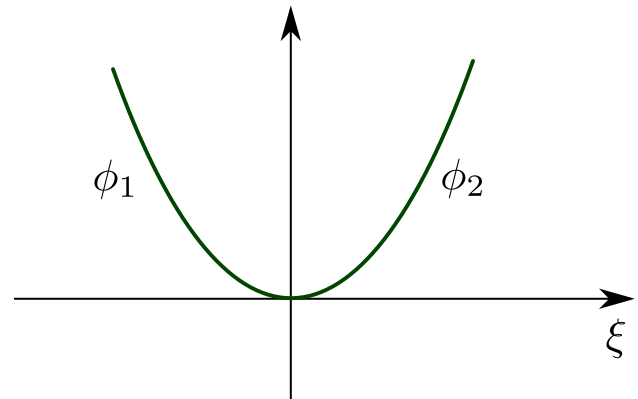
\includegraphics[scale=0.24]{assets/lectures_part_3-7a9fde69.png}
\end{gathered}
$$
\textbf{Тоді: } \fbox{$ f_{\eta} (y) =  \sum\limits_{i = 1}^{ n}{ f_{\xi} (\psi_i (y)) \cdot \left| \psi_i'(y) \right| \cdot \mathbb{I}_{E_{\varphi_i}}(y)}$}.
\end{boxteo}
\begin{proof}
  Розглядаемо множину B.
  $$  \int\limits_{B }^{ }{ f_{\eta} (y)dy} = \mathbb{P} \left\lbrace \eta \in B \right\rbrace =
 \mathbb{P} \left\lbrace \xi \in \phi_1^{-1} (B) \cup \cdots \cup \xi \in \phi_n^{-1} (B) \right\rbrace =
  $$
  $$
  =  \sum\limits_{i = 1}^{n}{ \mathbb{P} \left\lbrace \xi \in \phi_i^{-1} (B) \right\rbrace  }  - \text{ надалі доведення зводиться до попередньої теореми.}
  $$
\end{proof}
